\subsection{Warehouse Use-Case Results}
\label{subsec:warehouse_usecase_results}

After the controlled validation, the framework proposed is applied to simulate the warehouse digital twin application.
The simulation running on NR baseline configuration without ISAC components and NR ISAC configuration are evaluated for 2x2, 4x4, and 8x8 gNB array sizes.
Both scenarios use the same warehouse layout, wireless node positions, robot mobility model, radio parameters, and application workload, so the comparison isolates the effect of enabling situation awareness in the Sionna-backed channel.

\subsubsection{Warehouse Digital Twin}

To evaluate the framework in a realistic 6G warehouse environment, we created a digital twin application for warehouse.
The whole workflow is managed by the a warehouse controller.
The controller communicates with package sensors, racks, temperature and humidity sensors, mobile robots, video clients, and cameras.
The package sensors and racks are stationary, while the robots move between the package sensor area, the racks and dropoff area.
The sensors report the status to the controller periodically.
According to the status of the sensors, the controller sends commands to the robots to pickup the packages, put them on the rack or drop off at the dropoff area.
The controller track the positions of the robots by communicating with the gNB which keeps the positions of the robots in the system state.
The robots are equipped with cameras on them for monitoring the packages, the racks, and the environment and the user can request the video stream from the cameras through the video clients.

Among the warehouse devices, the package sensors, rack sensors, temperature and humidity sensors are stationary while the robots are mobile.
The robots are main targets for the ISAC evaluation because they are mobile, the propagation conditions change frequently, and the robot positions are tracked by the gNB.
Other wireless devices create background traffic and competing wireless flows.
Therefore, this scenario tests whether ISAC can improve robot communication while keeping the rest of the warehouse workload active.

The performance is evaluated in terms of application-related KPIs, propagation-related KPIs, power consumption related KPIs and sensing related KPIs.
First, application flows are grouped by node type to measure throughput, delay, jitter, and packet loss.
Next, Sionna propagation traces are grouped by device type to explain the channel behavior.
Then, energy traces are used to measure the power consumption of gNB according to the array size and ISAC activation.
Finally, the ISAC detected-object output is used to evaluate robot detection, tracking continuity, and localization error.

\subsubsection{Application-related KPIs}

The application results in Fig.~\ref{fig:exp2_app} are considered first because
they show the end-to-end effect experienced by the warehouse traffic. At
$2\!\times\!2$, ISAC does not yet provide a stable system-level benefit:
controller throughput drops from $417.674$~kbps to $205.345$~kbps, and
package-sensor throughput drops from $22.990$~kbps to $6.634$~kbps. Robot
throughput increases slightly from $1159.444$~kbps to $1249.326$~kbps, but this
increase is accompanied by $15.439\%$ packet loss, so the small-array ISAC case
is better interpreted as unstable delivery rather than a useful gain.

\begin{figure}[t]
  \centering
  
\includegraphics[width=\columnwidth]{images/exp2_app.png}
  \caption{Application-level KPIs under baseline and ISAC for the three gNB
    array sizes.}
  \label{fig:exp2_app}
\end{figure}

When the gNB array is increased to $4\!\times\!4$, the application behavior
changes because the ISAC configuration gains enough spatial resolution to
support the dominant mobile links. Controller and package-sensor throughput
return to the baseline range, while robot throughput increases to
$1582.081$~kbps compared with the baseline value of $1328.452$~kbps. The
$8\!\times\!8$ ISAC case keeps the same robot-dominant trend but reduces robot
throughput to $1445.378$~kbps, so the larger array does not provide a
proportional additional application gain. The application layer therefore
identifies $4\!\times\!4$ as the first array size where ISAC becomes useful for
the warehouse workload.

\subsubsection{Propagation-related KPIs}

The propagation results in Fig.~\ref{fig:exp2_prop} explain why the
application-level gain appears only after the array reaches $4\!\times\!4$.
For robot links, baseline path loss decreases from $83.948$~dB at
$2\!\times\!2$ to approximately $69.2$~dB at $4\!\times\!4$ and
$8\!\times\!8$. Under ISAC, the same trend is stronger: robot path loss falls
from $82.318$~dB at $2\!\times\!2$ to $57.359$~dB at $4\!\times\!4$ and then
remains almost unchanged at $8\!\times\!8$. This channel-level saturation
matches the application-level saturation, because most of the useful ISAC gain
is already obtained at $4\!\times\!4$.

\begin{figure}[t]
  \centering
  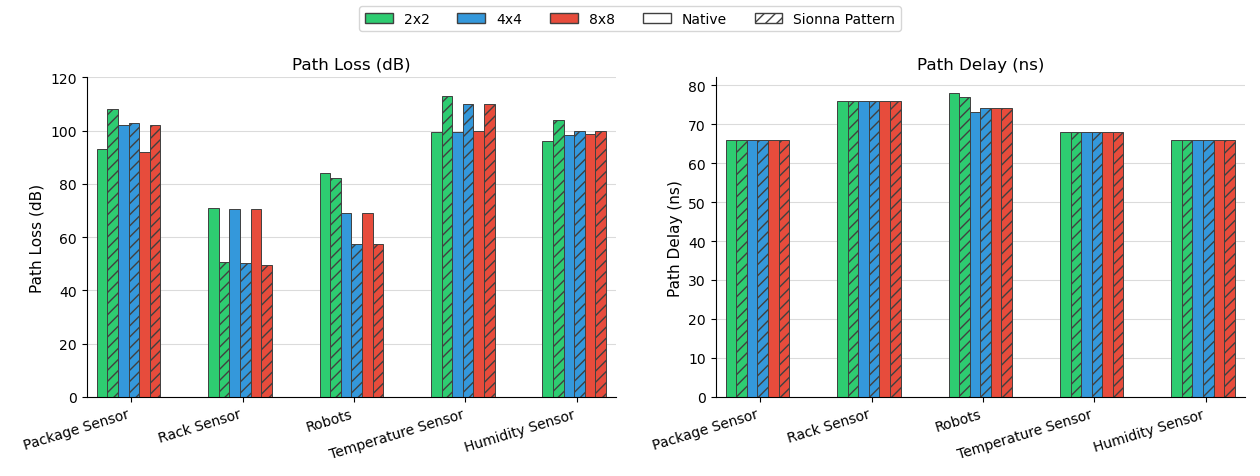
\includegraphics[width=\columnwidth]{images/exp2_prop.png}
  \caption{Propagation KPIs grouped by wireless node category, with solid bars
    for Native and hatched bars for Sionna Pattern.}
  \label{fig:exp2_prop}
\end{figure}

The propagation improvement is not uniform across all warehouse devices, and
this selectivity is important for interpreting the system result. Rack-sensor
links also benefit from ISAC, with roughly $20$~dB lower path loss than the
baseline across the tested array sizes. In contrast, package, temperature, and
humidity sensors experience higher path loss under ISAC than under the
baseline. The overall throughput improvement is therefore driven mainly by the
mobile robot links, which are the links most directly aligned with the
sensing-informed beamforming objective.

\subsubsection{Power Consumption related KPIs}

The power results in Fig.~\ref{fig:exp2_power} are evaluated after the
communication and propagation results because they determine whether the
observed gains are practically affordable. The dominant power factor is the gNB
array size rather than ISAC activation alone. The gNB average power rises from
approximately $25.6$~W at $2\!\times\!2$ to $51.3$~W at $4\!\times\!4$, and
then to about $145$~W at $8\!\times\!8$. The corresponding gNB energy increases
from about $3.1$~kJ to $6.15$~kJ and then to approximately $17.4$~kJ.

\begin{figure}[t]
  \centering
  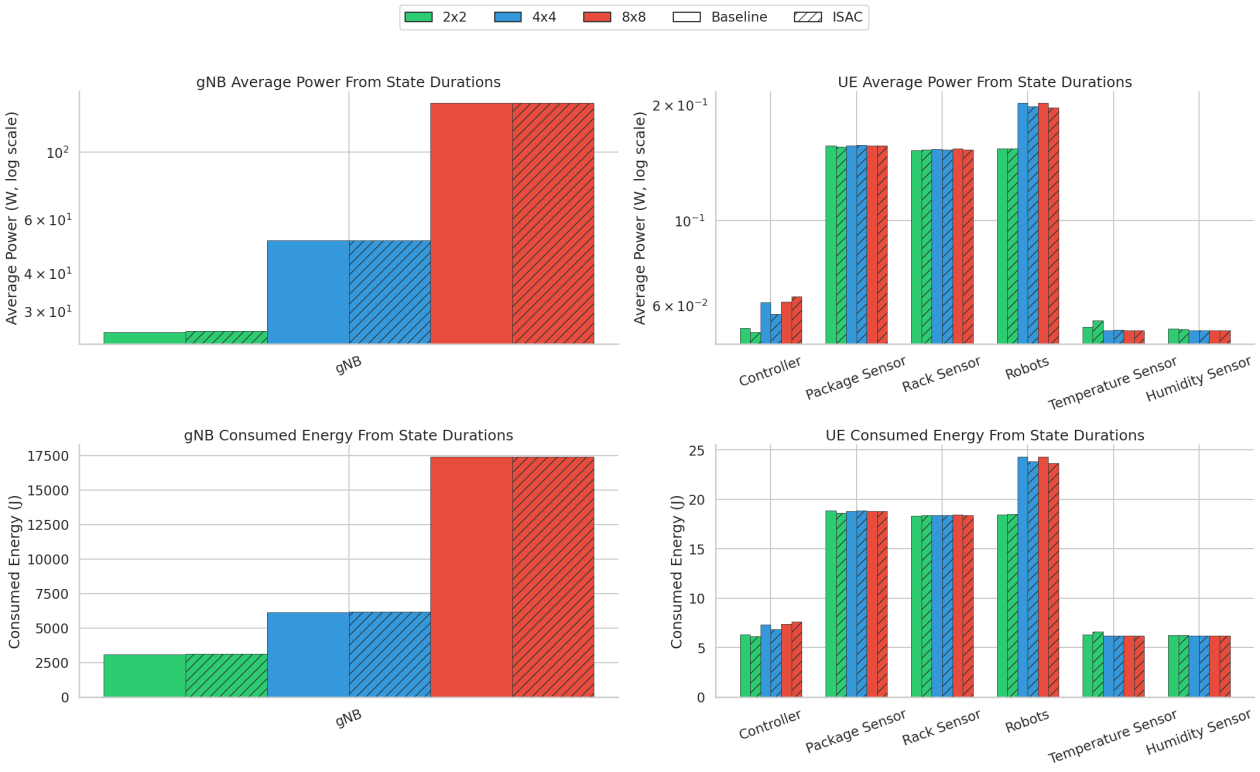
\includegraphics[width=\columnwidth]{images/exp2_power.png}
  \caption{Average power and consumed energy under baseline and ISAC.}
  \label{fig:exp2_power}
\end{figure}

This energy trend changes the interpretation of the larger array sizes. At the
system level, total reported energy is nearly identical between baseline and
ISAC for the $4\!\times\!4$ and $8\!\times\!8$ cases, while ISAC slightly
improves the useful throughput. However, the $8\!\times\!8$ array requires much
higher gNB power without giving a proportional communication gain over
$4\!\times\!4$. Therefore, the energy results reinforce the application and
propagation results: $4\!\times\!4$ is the balanced operating point for the
tested warehouse workload.

\subsubsection{Sensing and Localization}

The sensing results are evaluated last because they are available only in the
ISAC scenario and because they explain whether the communication gains are
supported by meaningful target awareness. Fig.~\ref{fig:exp2_sense} shows that
the main sensing improvement occurs when the gNB array is increased from
$2\!\times\!2$ to $4\!\times\!4$. The detection rate rises from $0.485$ to
$0.523$, and the missed-detection rate correspondingly falls from $0.515$ to
approximately $0.477$. The $8\!\times\!8$ case changes these values only
slightly, with a detection rate of $0.526$, so sensing also saturates after the
$4\!\times\!4$ configuration.

\begin{figure}[t]
  \centering
  
\includegraphics[width=\columnwidth]{images/exp2_sense.png}
  \caption{Sensing KPIs for the ISAC warehouse scenario.}
  \label{fig:exp2_sense}
\end{figure}

False positives and track continuity clarify the quality of those detections.
Validated false positives are already low at $2\!\times\!2$ and fall to zero
for both $4\!\times\!4$ and $8\!\times\!8$. Track continuity remains close to
unity across the three array sizes, which means that once a valid robot
detection sequence is formed, the exported identity remains stable. The larger
arrays therefore improve sensing mostly by increasing valid detection
opportunities and reducing unstable detections, not by fundamentally changing
the tracking behavior.

\begin{figure}[t]
  \centering
  
\includegraphics[width=\columnwidth]{images/exp2_loc_err.png}
  \caption{Localization-error distribution for the ISAC warehouse scenario.}
  \label{fig:exp2_loc_err}
\end{figure}

The localization-error distribution in Fig.~\ref{fig:exp2_loc_err} shows the
same stability effect from a different angle. The $2\!\times\!2$ configuration
has the lowest median error at $0.384$~m, but it also has the largest maximum
error at $10.427$~m. The $4\!\times\!4$ and $8\!\times\!8$ configurations have
slightly higher median errors of about $0.577$~m, but their maximum errors are
reduced to around $4.5$~m and their upper-tail errors are lower. Thus, the
larger arrays do not mainly improve pointwise median localization; instead,
they suppress large-error outliers and make the sensing output more stable.

Overall, the warehouse use-case experiment shows that ISAC benefit depends on
sufficient antenna-array support. The $2\!\times\!2$ ISAC configuration is not
stable enough for the mixed warehouse workload, whereas the $4\!\times\!4$
configuration improves the dominant robot communication links, improves sensing
stability, and avoids the much higher gNB power cost of $8\!\times\!8$. The
results therefore support $4\!\times\!4$ as the most balanced configuration
among the tested cases.
